\section{Validation and reproducible measurements}
\label{sec:experiments}

The experiments answer three separate questions: does the new arithmetic
agree with independent rules, does it improve deliberately dense
coefficient operations, and does that improvement appear in complete
scanner workloads? A fourth experiment measures finite-target witnesses
against the existing filters. Keeping these questions separate is
necessary to interpret the results correctly.

\subsection{Mathematical and integration checks}

The integrated suite passes all 74 test methods: the 41 original
regression tests, 11 dense-algebra tests, 11 finite-target tests, and
11 integration tests. The recorded complete run took 13.080 seconds.
The algebra tests include exhaustive multiplication in $R_r$ for
$r\leq2$, random dense and sparse multiplication through $r=8$,
homogeneous inputs through $r=9$, 700 abstract partition plans, and
explicit trace, extra-dot, nilpotence, invalid-plan, and positive-genus
cases. The expected values come from a direct scalar surface evaluator
that does not use the production transform.

The matching test enumerates all 2,879 triples of \emph{noncrossing}
matchings on $0,2,4,6,8$ endpoints and tries three seeded coefficient
pairs per triple, giving 8,637 comparisons. This is an exhaustive
enumeration of those matching triples with sampled coefficients; it is
neither an exhaustive enumeration of all morphisms nor of unrestricted
matchings. The abstract-plan tests and tests at actual scan stages cover
additional geometry. The general validity claim rests on the proofs in
Sections~\ref{sec:algebra}--\ref{sec:engineering}.

An additional independent check program verifies 2,100 associativity
identities using sampled quadruples of noncrossing matchings through
12 endpoints, including 405 positive-genus intermediate plans. It also
performs 8,768 crossing-transfer comparisons through frontier size 18.
These exercise all four source/target smoothing pairs, zero, one, and
two newly closed circles, support sizes 32 and 33 on opposite sides of
the transfer threshold, highest-index coefficients, and monotone
relabeling. The relabeling run records 572 shape-cache hits in each of
the two adapters. Associativity and relabeling test relationships between
operations, in addition to checking individual output formulas.

The grading audit performs 27,723 entry inspections and 31,674 monomial
inspections across eight fixtures with input, greedy, and selected seeded
random orders. All satisfy~\eqref{eq:qdegree}. As stated earlier, this
audit sees pre- and post-elimination stage complexes; the proof treats
the intermediate cancellation updates.

Integration tests compare complete ranks and homological degree
distributions, and exercise $d^2=0$, shape caches, tail elimination,
connected-sum factorization, competing scan workers, CLI option
propagation, certificate replay, certificate corruption, filter order,
exhausted search budgets, and the shared deadline. A mocked clock checks
deadline semantics without relying on a flaky wall-clock race. The
certificate checker has a distinct edge-traversal implementation and does
not reuse the search's arc-extraction or conjugation tables. These checks
increase confidence in the implementation; they are not a machine-checked
formalization or external peer review of the proofs.

\subsection{Host, timing scope, and provenance}

The measurements use CPython 3.12.14 on Linux x86-64 with an Intel Xeon
Platinum 8573C host. This is a shared container, so scheduling variation
is visible, especially at sub-millisecond scales. We report medians and
retain every sample. The plotted ranges are observed minima and maxima,
not confidence intervals. No fitted asymptotic exponent or significance
claim is inferred from these few measurements.

The archive preserves the exact baseline Git blobs, measured PD inputs,
crossing orders, random seeds, raw timing samples, output invariants, and
source hashes. The original source materialization carried one additional
terminal line feed per baseline file. Removing that byte recovers the
recorded Git blob hash for every one of the 40 baseline files. Benchmark
hashes continue to identify the bytes actually measured; the provenance
record explains this reversible byte difference. JSON parsing and imports
are excluded from timing, so that normalization changes neither the timed
algorithm nor the mathematical input. The provenance checks do not
silently relabel one set of measured bytes as another.

\subsection{Cold dense coefficient operations}

For $m=4,\ldots,11$, construct the matching of adjacent endpoint pairs and
sample two coefficient tables in $\End(a)=R_m$. The random seed is
202610071. For each size, the three implementations are run in a seeded
random order in each of five repetitions. A fresh algebra object and
fresh plan cache are used for each sample. Timing includes compilation
of the composition plan and the complete coefficient operation, while
excluding imports, input generation, and the preceding garbage collection.
Every implementation returns exactly the same output.

\begin{table}[htbp]
\centering\small
% Generated from archived measurements; do not edit by hand.
\begin{tabular}{rrrrrr}
\toprule
$m$ & Input supports & Baseline & Adaptive & Dense & Ratio \\
\midrule
4 & 4 / 9 & 0.057 & 0.069 & 0.103 & 0.82 \\
5 & 13 / 13 & 0.134 & 0.160 & 0.150 & 0.84 \\
6 & 30 / 38 & 2.354 & 0.257 & 0.229 & 9.15 \\
7 & 70 / 65 & 5.937 & 0.479 & 0.404 & 12.39 \\
8 & 124 / 127 & 19.455 & 0.915 & 0.839 & 21.26 \\
9 & 267 / 269 & 83.865 & 3.076 & 2.781 & 27.26 \\
10 & 515 / 506 & 368.195 & 7.144 & 5.447 & 51.54 \\
11 & 1019 / 1014 & 1377.909 & 11.749 & 12.720 & 117.28 \\
\bottomrule
\end{tabular}

\caption{Cold composition on sampled coefficient tables. Times are
median milliseconds over five repetitions. The last column is the
baseline/adaptive ratio for this primitive alone.}
\label{tab:dense}
\end{table}

\begin{figure}[htbp]
\centering
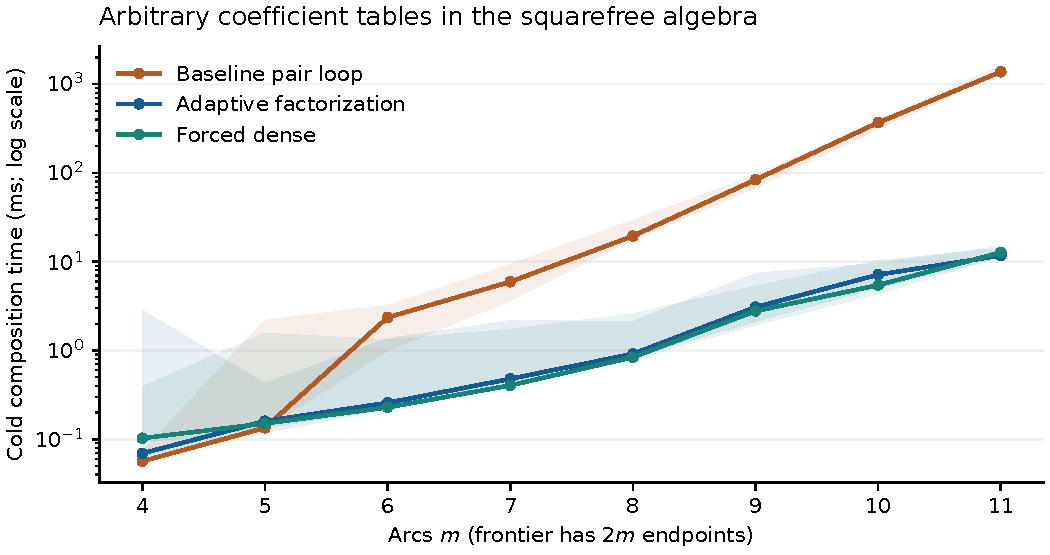
\includegraphics[width=.91\linewidth]{figures/composition_times.pdf}
\caption{The same cold-composition data on a logarithmic time axis.
Points are medians; shaded bands give the observed sample range.
The inputs are valid arbitrary morphisms, with no assertion that these
dense tables arise in the measured knot scans.}
\label{fig:dense}
\end{figure}

At $m=11$, the inputs have 1,019 and 1,014 supported terms. The baseline
populates 1,033,266 monomial-pair memo entries and takes a median
1.378 seconds. The adaptive implementation creates no such pair table and
takes 11.749 milliseconds, a measured factor of 117.28. The small
$m=4,5$ cases show the setup overhead instead. The large dense gain
supports the local algorithmic analysis, but the figure is not a
measurement of 117-fold faster knot recognition. The benchmark inputs
are deliberately general and need not be homogeneous; genuine scanner
entries have the additional structure of Proposition~\ref{prop:grading}.

\subsection{Paired complete scanner workloads}

The full-scanner experiment uses nine fixtures, three composition modes,
and five repetitions, for 135 completed timed scans. Every sample runs in
its own child process, performs one untimed warm-up, and then executes one
timed scan. The legacy process imports the original baseline; the adaptive
and dense processes import the integrated implementation. Each fixture
has one precomputed crossing order and one shape-cache setting, shared by
all modes. Imports, JSON parsing, diagram validation, and order selection
are outside the timed interval. All crossing transfers, cancellations,
rank calculations, and statistics are inside it.

\begin{table}[htbp]
\centering\small
% Generated from archived measurements; do not edit by hand.
\begin{tabular}{lrrrr}
\toprule
Fixture & $n$ & Legacy & Adaptive & Dense \\
\midrule
Trefoil & 3 & 0.388 & 0.566 & 0.464 \\
Figure eight & 4 & 2.373 & 1.153 & 0.737 \\
Conway & 11 & 6.140 & 6.486 & 7.047 \\
Kinoshita--Terasaka & 11 & 8.026 & 9.865 & 11.560 \\
Hard unknot 8 & 8 & 0.863 & 1.339 & 2.424 \\
$T(3,5)$ & 10 & 6.273 & 4.803 & 6.086 \\
$T(3,7)$ & 14 & 11.130 & 10.156 & 12.147 \\
Generated hard unknot 27 & 27 & 16.912 & 25.202 & 33.348 \\
Stress braid5 36 & 36 & 455.644 & 478.966 & 502.907 \\
\bottomrule
\end{tabular}

\caption{Complete scanner medians in milliseconds. Every one of the
135 runs agrees on total rank and the complete homological degree
distribution. These timings use a different, isolated-process protocol
from Table~\ref{tab:quotient}.}
\label{tab:scanner}
\end{table}

The operation counters explain the result more usefully than a selected
speedup number. On all nine fixtures, the adaptive mode selects zero
dense compositions and zero dense transfers. Their maximal frontiers
are at most eight endpoints, where coefficient tables are small. For
example, the 36-crossing stress input reaches 17,694 objects before
elimination and 5,898 afterward, but its maximum frontier is eight.
That workload is dominated by objects, entries, and sparse operations.
The dense asymptotic improvement has no opportunity to dominate there.

Adaptive/legacy median time ratios are 1.056 for Conway, 1.229 for
Kinoshita--Terasaka, 1.490 for the generated 27-crossing hard unknot, and
1.051 for the 36-crossing stress braid. Apparent gains on some small
fixtures are not robust evidence: the figure-eight legacy samples range
from 0.590 to 4.099 milliseconds. These measurements support leaving
\texttt{legacy} as the default. They also identify the next engineering
task: reduce adapter overhead on sparse entries, and find or generate
genuine scan stages whose graded coefficient layers are large enough to
test the new asymptotic regime.

\subsection{Finite-target search and existing filters}

The finite-target comparison uses one untimed warm-up followed by nine
warm repetitions. Search time includes arc extraction, greedy seed-plan
construction, assignment search, and independent certificate replay.
Imports and fixture JSON parsing are excluded. All rows use the same
fixture bytes for the compared procedures. Raw Khovanov time here is a
fallback comparator from this experiment; it must not be mixed with
the isolated full-scanner medians in Table~\ref{tab:scanner}.

\begin{table}[htbp]
\centering\small
% Generated from archived measurements; do not edit by hand.
\begin{tabular}{lrrrrr}
\toprule
Fixture & $b$ & $a$ & $A_5$ seeds & Default & Raw Kh \\
\midrule
Conway & 3 & 57 & 0.781 & 0.645 & 5.516 \\
Kinoshita--Terasaka & 3 & 67 & 0.492 & 0.739 & 6.266 \\
Hard unknot 8$\dagger$ & 2 & 18 & 0.111 & 0.403 & 1.402 \\
$T(3,5)$ & 3 & 35 & 0.549 & 0.155 & 4.281 \\
Stress braid5 36 & 4 & 820 & 7.361 & 0.420 & --- \\
\bottomrule
\end{tabular}

\caption{Warm median milliseconds. $b$ is the discovered seed count and
$a$ the number of complete seed-orbit assignments tried. $\dagger$ marks
an inconclusive $A_5$ search, which has not decided the unknot.
An em dash means that comparator was not measured.}
\label{tab:quotient}
\end{table}

For Conway and Kinoshita--Terasaka, the seed plans use three arcs and find
certificates after 57 and 67 orbit assignments, respectively. Both
certificates have image group of order 60. The seed searches take
0.781 and 0.492 milliseconds, compared with 5.516 and 6.266 milliseconds
for the raw homology fallback in the same protocol. These are useful
fallback savings on those two fixtures. The existing complete recognizer,
however, already rejects both through its Jones stage in about
0.645 and 0.739 milliseconds. The new filter therefore belongs after
the cheap existing obstructions and remains disabled by default.

The 36-crossing stress braid supplies a second caution. The seed search
takes 7.361 milliseconds and finds an image of order 12; the existing
default pipeline takes 0.420 milliseconds. The alternative arc-consistency
solver takes 665.067 milliseconds on that fixture. Search heuristics can
make a large difference even with the same finite target, but beating
another search procedure does not imply beating the recognition pipeline.

For the hard eight-crossing unknot, the seed solver exhausts 18 orbits in
0.111 milliseconds and returns \texttt{INCONCLUSIVE}. Comparing that
time as if it were an unknot decision would be invalid. The separate
$T(3,7)$ control exhausts all 231 seed orbits and likewise stays
inconclusive, as required by the proven $A_5$ obstruction. The constraint
solver also returns inconclusive after 182 search nodes. The archive
includes the certificates for successful cases, the seed plans, and both
exhaustive $T(3,7)$ search records.

\subsection{What the evidence establishes}

The proved local bound, the independently reproduced algebraic identities,
and the dense benchmarks agree. The ordinary full-scanner measurements
show that the missing performance theorem concerns much more than that
primitive. The finite-target backend provides cheap, replayable witnesses
on selected instances, while its negative controls confirm the need for
an exact fallback. No experimental result here establishes a bound on
$b$, $N$, or $Q$ for all knots, a generic advantage from enabling the new
modes, or an unrestricted quasi-polynomial recognizer.
